\chapter{Full text Search}
\label{chap:fulltext}

The amount of information has grown rapidly in the last few years due to the information explosion caused mainly by the World Wide Web. 
The result is that nowadays, people are exposed to much more information than they used to be. 
In order to manage such amount of data and obtain relevant information very quickly (in the order of milliseconds), new powerful techniques operating on vast collections of data were needed.
The aim of this chapter is to explain basic concepts applied in full-text search, one of the methods dealing with the problem of searching information.

%Information and efficient access to it form an essential part of life in a modern society. 
%Computing and related technologies have changed the ways textual information is stored, searched and retrieved. 
%The amount of information has grown rapidly in the last few years due to the information explosion caused mainly by the World Wide Web. 
%The result is that nowadays, people are exposed to much more information than they used to be. 
%Simple categorization of documents made by humans, although doable, is no longer an efficient method of storing data to be searched. 
%Except for the fact that this activity is very time-consuming, it can also be automated. 
%In order to manage such amount of data and obtain relevant information within a reasonable time period, new powerful techniques operating on vast collections of data were needed.
%
%The problematics of searching relevant information in large data sets has been an objective of a detailed research for more than sixty years. 
%The aim of the following parts is to introduce some fundamental concepts of information retrieval, a discipline including the full text search, in the context of full text search and compare these concepts with similar principles used in the relational and
%NoSQL database worlds.
%
%The latter chapter describes available open-source full text search engines.


\section{Information retrieval}



%%% -------- ZDROJE -----------------------

% en.wikipedia.org/wiki/Information_retrieval

% http://en.wikipedia.org/wiki/Full_text_search

% http://www.sigir.org/forum/2005J/buntine_sigirforum_2005j.pdf?searchterm=lucene - kapitola 3!!!

% http://www.lovdata.no/litt/hand/hand-1991-2.html - HODNE DOBRY! (precision-recall graf)

% http://people.ischool.berkeley.edu/~hearst/irbook/1/node5.html

% http://www.sigir.org/museum/pdfs/Report_on_the_Testing_and_Analysis_of_an_Investigation_Into_the_Comparative_Efficiency_of_Indexing_Systems/pdfs/p95-chapter_10.pdf?searchterm=information+retrieval

% http://openlib.org/home/krichel/courses/lis618/readings/rijsbergen79_infor_retriev.pdf - Rijsbergen

% http://nlp.stanford.edu/IR-book/pdf/10xml.pdf - cast Introduction

% http://hughewilliams.com/2012/03/24/compression-speed-search-engines/

% http://searchhub.org/2009/09/02/full-text-search-engines-vs-dbms/

% http://www.ideaeng.com/database-full-text-search-0201

% http://lingpipe-blog.com/2008/11/22/lucene-or-a-database-yes/

% http://www.sai.msu.su/~megera/postgres/fts/doc/fts-whatdb.html

% http://nlp.stanford.edu/IR-book/html/htmledition/irbook.html

% http://books.google.cz/books?id=_fGvneZhwrQC&pg=PA10&hl=cs&source=gbs_toc_r&cad=4#v=onepage&q&f=false

%%% ------------------------------------



Full-text search can be considered as a part of a subdiscipline of computer science known
as \textit{information retrieval} (IR) \cite{Witten:1999:MGC:323905}.
There is a number of available definitions of information retrieval.
According to \cite{IRDataAlgorithms}, information
retrieval (IR) is loosely defined as

	\begin{quote}
		\textsl{``the subfield of computer science
	that deals with the automated storage and retrieval of documents''}
	\end{quote}

This definition as well as the definitions from other sources (e.g. from \cite{Witten:1999:MGC:323905}) sum up the purpose of IR in a very general way.
%While the definition above puts no restrictions on the nature of stored documents in the IR system and therefore comprises both full-text search and database systems, there exist stricter IR definitions that do not apply to structured data found typically in relational databases. 
There also exist stricter IR definitions that explicitly mention working with unstructured data.
One such definition of IR can be found in \cite{ManningRaghavanSchuetze08}:

	\begin{quote}
		\textsl{``Information retrieval (IR) is finding material (usually documents) of an unstructured nature (usually  text) that satisfies an information need from within large collections (usually stored on computers).''}
	\end{quote}

All IR systems - and full-text search engines are no exception - are based on the same architecture described in Section \ref{fullTextArch} which is adapted to requirements that the specific systems have. In addition, these systems share common IR terminology, whose most important terms are explained in this chapter.

\section{Principles of Full-text Search}

% Ostry text

The field of full-text search covers a wide range of topics, including efficient algorithms and data structures that enable fast and reliable full-text search over large amount (in practice gigabytes) of data. 
It is not the aim of this thesis to provide a deeper, more complex insight into this problematics as the final implementation of the full-text search feature will be based on an existing full-text search engine. 
However, there are several terms and concepts that must be at least briefly explained so that the reader can fully understand the latter text.


\subsection{Full-text Search Engine Architecture}
\label{fullTextArch}

As can be seen in schema in Figure \ref{fig:fulltext_schema}, full-text search engines comprise several steps in order to provide a user with search results to a given \textsl{query}. 
\textsl{Query} is in this case a text phrase, optionally enriched by special operators which serve for refining the query. 
It is a \textsl{user} of the IR system who comes up with the query, expecting that the system will fulfill his or her \textsl{information need} by returning relevant search results.

\subsubsection{Documents}

Search engines need to ingest source data first to have something to searching on. 
The basic informational unit which is processed by the search engine and returned to the user in case of match with the query is called \textsl{document}. 
Documents consist of one or more fields with content.
In this context, documents inserted to the system are representations of real documents, such as HTML, PDF files or relational database data.
Therefore, a series of data transformations must be made first in order to extract all desired searchable information from different data sources. 
These transformation steps are discussed in the practical part of the thesis in Chapter \ref{chap:implementation} and are for reasons of clarity not depicted in the schema. 
% Each document is typically identified by a unique \textsl{document ID}.
  
\begin{figure}[h]
	\centering
		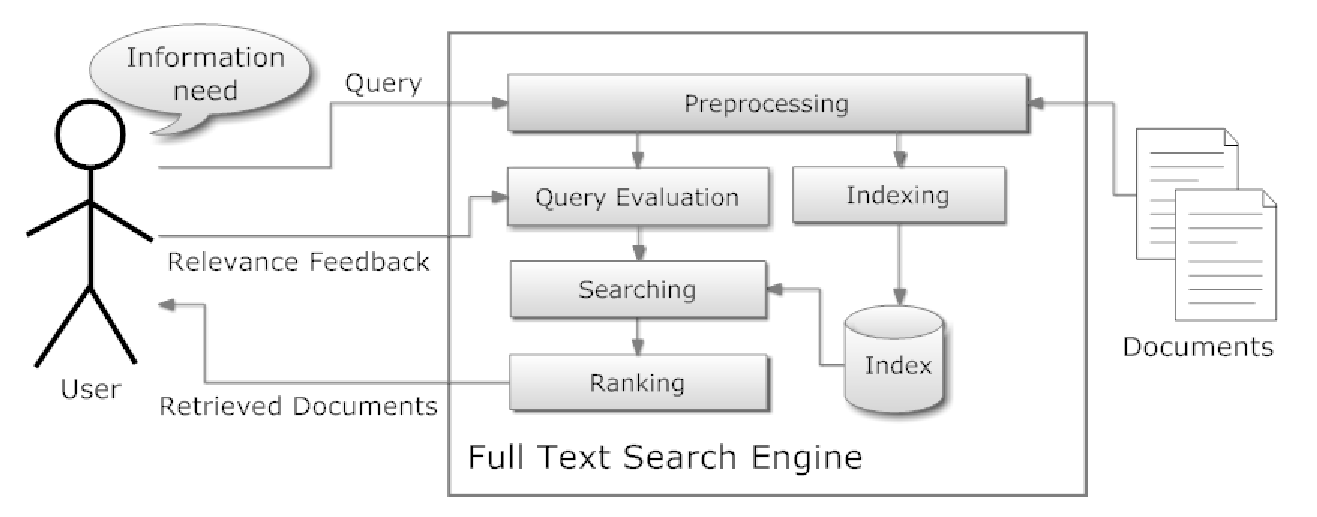
\includegraphics[width=1.00\textwidth]{figures/fulltext_schema.eps}
	\caption{IR Architecture Schema. Adapted from \cite{IR:ImplemEvalSearchEng,MiddletonBaeza}.}
	\label{fig:fulltext_schema}
\end{figure}

\subsubsection{Preprocessing}

Both input query and documents usually undergo several preprocessing steps.
These steps transform the original query or document content to searchable text units called \textit{terms}.
If documents are processed, the created terms are then together with document metadata passed on for indexing.
It is important to mention that in order to get correct results, the same preprocessing steps must be applied for both search queries and documents.

The first preprocessing step is called \textit{tokenization}.
During the process of tokenization, the document content is treated as a character stream.
It is broken into basic elements called \textit{tokens}, in some sources also referred to as \textsl{words}, by using appropriate \textit{tokenizers}.
Tokenization happens typically at the word level, so a token can be seen as a simple word of ordinary text in most cases.
Apart from the obvious creation of tokens by splitting the input stream by the whitespace characters, tokenizer implementations also remove punctuation and may include more sophisticated strategies that are oriented to a given problem domain \cite{ManningRaghavanSchuetze08}.

% stop words
After a token stream is created, those tokens that bring no or very little information are often filtered out, thus not indexed.
These tokens, mainly articles, prepositions and conjunctions, such as \textit{``the''}, \textit{``an''}, \textit{``to''}, \textit{``and''} etc. are normally called \textit{stop words} and are included in the so-called \textit{stop list}.
Although eliminating tokens listed in the stop list can reduce the final index size and speed up processing, it will disable finding phrases made of stop words only, such as \textit{"to be or not to be"}.

% token normalization
The next step concerns \textit{token normalization}. 
It is a process that includes token transformations, such as \textit{case-folding} (converting all letters to their lowercase equivalents or vice versa), removal of accents and diacritics etc.
The output of token normalization is the creation of \textit{equivalence classes}. 
The equivalence classes ensure that \textit{``matches occur despite superficial differences in the character sequences of the tokens''} \cite{ManningRaghavanSchuetze08}.

% stemming
Sometimes it is useful to retrieve documents containing not only an exact searched keyword, but also one of its possible variations, such as \textit{walk}, \textit{walks}, \textit{walking}, \textit{walked} for the keyword \textit{walk}.
The corresponding transformation based on reducing words to their root forms (or \textit{stems}) is known as \textit{stemming}.
One of the stemming positive side-effects is a decreased index size due to storing only the created stems in the index.
Using stemming, however, may lead to obtaining false positives, if different words are assigned the same stem, or false negatives, if different forms of the same word get different stems assigned.
There are several stemming algorithms available and more information about them can be found e.g. in \cite{IRDataAlgorithms}.

%synonyms
It is also possible to do \textit{synonym expansion} of tokens. The synonym expansion can be triggered either during indexing, or during querying. Similarly to defining stop words, synonyms are stored typically in a \textit{list of synonyms}.
The usage of synonyms is very domain-specific, so irrelevant query results might be obtained if the usage of synonyms is not optimized.

% Indexovani
\subsubsection{Indexing}

Indexing deals with effective storage of created document terms.
Therefore, indexing involves transformation of documents to a more convenient data structure for the needs of information retrieval - the \textit{index}.

% HOTOVO
\subsubsection{Index}

Index is defined by Frakes \cite{IRDataAlgorithms} the following way: 
	\begin{quote}
	\textsl{``A collection of terms with pointers to places where information about them can be found.''} 	
	\end{quote}
Based on information found in \cite{Witten:1999:MGC:323905, IRDataAlgorithms, ManningRaghavanSchuetze08}, there are three main methods of indexing – \textit{inverted index}, \textit{signature file} and \textit{bitmaps}. Based on the comparisons made in \cite{Witten:1999:MGC:323905} and in \cite{Zobel:1996:GPC:234889.234891}, using inverted indexes should be the preferred way due to their search efficiency and lower index size they require. The remaining two alternatives are recommended to be used only in certain circumstances which are very rare in practice. 

\subsubsection{Inverted Index}

This data structure, sometimes referred to as the \textit{inverted file} \cite{IRDataAlgorithms}, can be thought of as the well-known index at the end of a book. 
It consists of a \textit{vocabulary} (sometimes also called as \textit{lexicon}) of indexed terms.
If the IR terminology is followed, the inverted index can be characterized more precisely. One of such more precise characteristics can be found in \cite{Witten:1999:MGC:323905} and claims that:

\begin{quote}
		\textsl{``An inverted file contains, for each term in the lexicon, an inverted list that stores a list of pointers to all occurrences of that term in the main text, where each pointer is, in effect, the number of a document in which that term appears.''}
	\end{quote}
	
	To visualize the basic idea of the inverted index, Figure \ref{fig:inverted_index} shows a few indexed terms in the dictionary and their corresponding \textit{inverted lists} (also known as \textit{postings lists} \cite{IR:ImplemEvalSearchEng}).
	Inverted lists contain typically document identifiers that point to documents themselves.
	Inverted indexes are usually stored in a highly compressed form on disk and this why many index compression techniques targeted to their compression have been studied \cite{Zhang05efficientquery}. 

\begin{figure}[h!]
	\centering
		\includegraphics[width=1.00\textwidth]{figures/inverted_index.eps}
	\caption{Inverted Index Schema. Adapted from \cite{ManningRaghavanSchuetze08}.}
	\label{fig:inverted_index}
\end{figure}

% index granularity
	
\subsubsection{Query Processing, Searching and Ranking}

In addition to the steps done in the \textit{processing} phase, a query based on the usage of an inverted index must go through the following three steps \cite{MiddletonBaeza}:

\begin{enumerate}
	\item The query terms are searched in the index vocabulary.
	\item From each term found in the vocabulary, all the posting lists are retrieved and decoded.
	\item The lists are then manipulated so that results of the query are received.
\end{enumerate} 

The type of manipulation depends on the type of the used model of information retrieval.

% boolovsky model - princip
In the case of the \textit{Boolean model}, the query terms are combined with three basic Boolean operators - intersection (AND), union (OR) and difference (NOT).
% co vraci
\textit{``The answers, or responses, to the query are those documents that satisfy the stipulated condition.''} \cite{Witten:1999:MGC:323905}.
% nevyhody
This model suffers from several disadvantages.
First, it is difficult for many users to formulate correct Boolean queries in order to get expected results \cite{Salton:1989:ATP:77013}. 
%Thus, creating non-trivial queries can be complicated.
Furthermore, only exact matches are retrieved (document either matches the Boolean expression or not) and all terms are equally important, so the model gives no information about relevance of retrieved documents. 
 
%term weights - co to je a proc se o tom zminuju
More advanced retrieval models use \textit{term weights} which provide additional information about importance of individual terms in the documents.
The weights are derived from statistical information about a term, usually by calculating the \textit{term frequency} (the number of occurrences of a term in a document) and \textit{inverse document frequency} (the inverse-like value of the number of documents that contain a specific term) for each query term contained in a document.
More information about term weight calculation can be found e.g. in \cite{hiemstra2001using,ManningRaghavanSchuetze08}

%obrazek
\begin{figure}[h!]
	\centering
		\includegraphics[width=0.70\textwidth]{figures/vectorspace.png}
	\caption{\textit{A query and document representation in the vector space model.} Adapted from \cite{hiemstra2001using}.}
	\label{fig:vectorspace}
\end{figure}

% vector space model
One of the retrieval models using term weights is the \textit{vector space model}. 
This model represents queries and documents as vectors in a multidimensional vector space, in which each dimension belongs to one term.
The final vector size and orientation is composed of individual term weights for each dimension (see Figure \ref{fig:vectorspace}).
The vector sizes and angles between them can be then compared by using appropriate similarity measures.
%Probably the most popular similarity measure is the \textit{cosine similarity}.
Consequently, measuring similarity of a query vector and found document vectors enables \textit{ranking} of the query results.

% probabilistic mode
Another IR model used in practice by several search engines is the \textit{probabilistic model}. 
This model is based on probabilistic theory and its more detailed explanation, which is out of scope of this work, can be found e.g. in \cite{van1979information}. 

% \subsubsection{Ranked query}


% \subsubsection{Ranking}	



% \subsubsection{Relevance Evaluation}

% precision, recall



%  vs. DB: Nevertheless, Lucene only deals with a single, built-in data model -- the Document class, which is too simple to describe those complex relationships. 

% Poznamky

%An IR system matches user queries - formal statements of information
%needs - to documents stored in a database. {[}IRDSA,Frakes{]}
%
%An IR system must support certain basic operations. There must be
%a way to enter documents to a database, change the documents and delete
%them.The must be also some way to search for documents, and present
%them to a user.
%
%Though it is possible to keep the index structure in main memory,
%in practice IR databases are usually stored on disk because of their
%size.
%
%
%The basic item stored in the index 
%
%Todo Lucene in Action and other sources
%
%identify index terms
%
%how to decide if a document matches a query
%
%precision = number of relevant documents retreived divided by the
%total number of documents retreived
%
%recall = number of relevant documents retreived divided by the total
%number of relevant documents
%
%ideally, both parameters should equal to one. This would mean that
%the system returns all relevant documents without introducing any
%irrelevant documents in the results set - impossible to acheive in
%practice.
%
%Improving recall -> precision decreases, likewise improving precision
%at the expense of recall
%
%Furthermore - tradeoff between retreival effectiveness and computing
%cost (key word matching < statistical ranking <\ natural-language
%processing)
%
%Statistical model
%
%Here a document is conceptually represented by a vector of keywords
%extracted from the document, with associated weights representing
%the importance of the keywords in the document and within the whole
%document collection.
%
%Query is modelled as a list of keywords with associated weights representing
%the importance of the keywords in the query.
%

\section{Full-text Versus RDBMS Searching}
\label{sec:fullVsDb}

% \subsection{Structure}
% jak se fulltext lisi oproti databazi
% kdy jej pouzit a uvest proc databaze ne

% http://blog.griddynamics.com/2011/04/indexes-rdbms-vs-coherence-vs-lucene.html

% http://use-the-index-luke.com/sql/where-clause/searching-for-ranges/like-performance-tuning

% Relational database define the structure of stored data on the table level.
% Related data contained in multiple tables can be referenced to and they also can be retrieved as a single piece of data by using SQL (Structured Query Language) JOIN operation.
% Most of them also enable transactional processing by guaranteeing four properties known under the acronym of ACID which stands for Atomicity, Consistency, Isolation and Durability \cite{Gray:dbTransactions}. 

% The index in full-text search engines can be seen as a single table from the relational database perspective.
% It contains a collection of documents, consisting of fields with their values.
% Documents roughly correspond to table records.

%Compared to relational databases, data structure is in some implementations set on the document level, some implementations require to have a single document structure defined on the index, table-like level.
% However, document structure is usually flat and 
% index odpovida tabulce v rel db, dokument odpovida radku v tabulce
% data denormalizovana



%LIKE expressions starting with a wildcard cannot use an index to locate the matching entries. 
%There is no simple way to tune such a query. 
%Use another access path if possible (e.g., additional where conditions). 
%Otherwise consider using a full-text index. 

% \subsection{Searching}

Relational Databases (RDBMS) are %the most popular type of available databases. 
a proved solution to storing large volumes of structured data, in which they excel.
As long as there is no need to search in a lot of data stored in a RDBMS, relational databases are a recommended solution for our domain.
However, the usage of a classical RDBMS to search a phrase in a block of text, for example in a text column, may become unacceptable due to too much time needed to scan a huge amount of data.
Traditional search engines offer the SQL (Structured Query Language) \texttt{LIKE} operator. 
The \texttt{LIKE} operator is used for searching a given pattern in a specific column.
When using \texttt{LIKE}, full table scan is needed to be performed \cite{ali2011sphinx}. 
It means that each row is examined to check if it matches the searched string or not. 
With the increasing amount of data in the table, it takes more time to process them by the full table scan.

Another disadvantage of using SQL queries containing the \texttt{LIKE} operator is the fact that if more terms are searched, the associated SQL query grows in complexity.
Since it is intended to store normalized data in RDBMS to avoid data redundancy and ensure their consistency, searched data are often stored in multiple tables.
This is why multiple JOIN operations must be used to fetch all data from the corresponding tables.
Furthermore, the query must be written the way to ensure finding the records with terms not necessarily next to each other, too. 
As the query gets more complex, it therefore takes more time to get query results.
Another reason why the query execution slows down is that the query needs to match each term individually.

It is important for a user to know how much the found results match the input query. 
RDBMS simply output the records matching the criteria.
This way the found results of the output result set do not contain any information about the relevancy to the searched terms. 

Full-text search engines, on the other hand, use different data structures especially designed for full-text searching needs.
If there is a lot of data to be searched, inverted index provides a fast way to return matching documents by looking up the corresponding terms in the index dictionary which point to the target documents.
% Jak vypadaji dokumenty
Documents are usually stored in a denormalized form, meaning that there may exist duplicate, redundant information across the document collection.
In this aspect they are more similar to NoSQL document-oriented databases, such as MongoDB.
While MongoDB allows creating hierarchical structures by nesting a document as a field value of another document, this cannot be achieved in full-text documents, mainly due to increasing the retrieval speed.
Furthermore, by using methods described in section \ref{fullTextArch}, full-text search engines output ranked search results that do not have to match the input query completely.

%Next, caching support is available for most of the search engines for further searching acceleration. 
%This way, the index and the most frequent search results are loaded into memory.
% Compared to RDBMS, index structure of search engines is more granular.

%Zdroj: \cite{Solr3EnterpriseSS}

% nize jsou SRACKY

%Full text search engines are based on the document structure which is analogous to a single table in RDBMS. 
%Compared to RDBMS, there is in most cases no JOIN or any similar operation. 
%The overall structure of documents is flat due to the need to retrieve stored data as fast as possible.
%
%
%On the contrary, IR systems provide us with additional relevancy information of searched terms. 
%Document relevancy is one of the key features of full text search engines because it is desired to display the results sorted by their relevance (mostly those most relevant ones are displayed first).
%
%It is worth mentioning that some DBMS possess native full-text support.
%MySQL - keyword FULLTEXT INDEX, for searching on a field, on which full text search will be performed. 
%These full text indexes are supported only by MyISAM engine \cite{MyISAM}. 
%They are generally faster than LIKE, however, their usage is limited - vendor lock-in,
%moreover, this solution is not unified (various implementations and syntaxes can differ, decision to switch to another database could mean interactions to the current system to preserve functionality and scalability. 
%It is bound solely to DBMS - they also lack bigger scaling possibilities and have problems in this area. 
%And it is still slower than external search engines.
%
%{[}IRDSandA,Frakes, p.14{]}:
%
%difference - amount of usable structure in their data objects. Document
%generally have less usable structure than the table used by relational
%DBMS.
%
%IR - retrieval is probabilistic. 
%No certainty that a retrieved document will meet the information need of the user. 
%(typically, some relevant documents will be missed, whereas some irrelevant documents will be
%retrieved) vs. DB queries consist of attribute-value pairs that either
%match or do not match records in the database.
%
%same - their databases are often very large (can be gigabytes)
%
%same - database volatility - means constant changes as documents are
%added, changes or deleted.


%\subsection{Benefits of full text search}
%
%When searching over unstructured data and large data sets, full text
%search should be favored to querying relational databases.
%\begin{itemize}
%\item faster than traditional database search - benefits from word index,
%which is traversed during searching (they are used to look up records),
%vs. DB - full table scan is performed- see the section \ref{sec:fullVsDb}
%\item found records can be sorted by their relevance. This is called ranking.
%\item good performance also over a DB with millions of records
%\item ability to skip common words with no additional information. This
%depends on the domain languages (in case of English these words include
%e.g. the, an, for), search precision can decrease in some cases. 
%\end{itemize}
%It is advised to use full text search if:
%\begin{itemize}
	%\item there is a lot of unstructured data that are to be looked up
	%\item it is necessary to get optimized search results.
	%\item flexible querying is demanded.
%\end{itemize}


%\cite{Fox:1991:FFA:903195}
